\section{Two scale preconditioner}

Let us finally move on to the two-scale preconditioner. We showed in the previous part that using only the fine scale preconditioner was not a good idea when the number of quadrants increased (the number of iterations roughly doubles when the mesh size is divided by two). As explained in the theory chapter, the idea is to add a coarse part in the preconditioner (i.e. $P = P^f + P^c$), consisting mainly of solving a problem with an interpolation degree $p=1$ with a geometric multigrid method, so that the number of iterations stays constant when we increase the number of quandrants.  

As in the previous section, the tests will be performed in two parts : first, we will analyse the performances of the two-scale preconditioner when there are no hanging nodes (but for both regular and distorted meshes) and then we will look at what happens when the forest of quadtrees is refined recursively and therefore the mesh is not conforming anymore. 

\textcolor{red}{Ajouter si on fait le truc avec les erreurs et le temps}

\subsection{No hanging nodes}

Let us first present the problem we will solve in this part. We want our numerical solution to capture both low and high frequency modes so we will superpose a cosine with low frequency and a sine with a high frequency. As before, the domain is : $\Omega = \left[ -1;1 \right]^2$ and $\Gamma$ is the boundary. We will solve : 

\begin{align}
\nabla^2 u &= -\frac{\pi^2}{2}\cos(\frac{\pi}{2}x)\cos(\frac{\pi}{2}y) - 5\pi^2\sin(5\pi x)\sin(5\pi y) &\text{on $\Omega$} \label{eq:prob_two}\\
u &= 0  &\text{on $\Gamma$}
\end{align}

This problem has an analytic solution that is given by : 

$$ u(x,y) = \cos(\frac{\pi}{2}x)\cos(\frac{\pi}{2}y) + \frac{1}{10}\sin(5\pi x)\sin(5\pi y)$$

\begin{figure}
\centering
\includegraphics[scale=0.35]{Results/two_simple_sol.eps}
\caption{Numerical solution to problem \ref{eq:prob_two} using an interpolation of order $p=2$ and $1.0\:10^{6}$ degrees of freedom on a regular mesh with no hanging nodes. This numerical solution has been obtained by the PCG with the two scale preconditioner.}
\label{two_simple_sol}
\end{figure}


An example of a numerical solution obtained using the preconditioned conjugate gradients with the two scale preconditioner can be seen on figure \ref{two_simple_sol}. This solution has been obtained in only 8 iterations and with an interpolation of degree $p=2$. 

\subsubsection{Regular meshes}

Let us now look at what happens to the number of iterations when we decrease the mesh size for different degrees of interpolation. Table \ref{two_table_reg} shows the number of degrees of freedom for the different meshes used (indeed, for a given mesh, the higher the degree of the interpolation, the more global nodes we have). We can already see that, thanks to the coarse preconditioner, we are able to have a lot more degrees of freedom than in the case where we only had the fine preconditioner.

\begin{table}
\centering
\begin{tabular}{c|cccc}
\hline
Number of quadrants & $128^2$ & $256^2$ & $512^2$ & $1024^2$\\
\hline
$p=2$ & $6.6\:10^4$ & $2.6\:10^5$ & $1.1\:10^6$ & $4.2\:10^6$ \\
$p=4$ & $2.6\:10^5$ & $1.1\:10^6$ & $4.2\:10^6$ & $1.7\:10^7$ \\
$p=6$ & $5.9\:10^5$ & $2.4\:10^6$ & $9.4\:10^6$ & $3.8\:10^7$ \\
$p=8$ & $1.1\:10^6$ & $4.2\:10^6$ & $1.7\:10^7$ & $6.7\:10^7$ \\
\hline
\end{tabular}
\caption{Number of degrees of freedom for a regular mesh with different number of quadrants and for different degrees of interpolation.}
\label{two_table_reg}
\end{table}

\begin{figure}
\centering
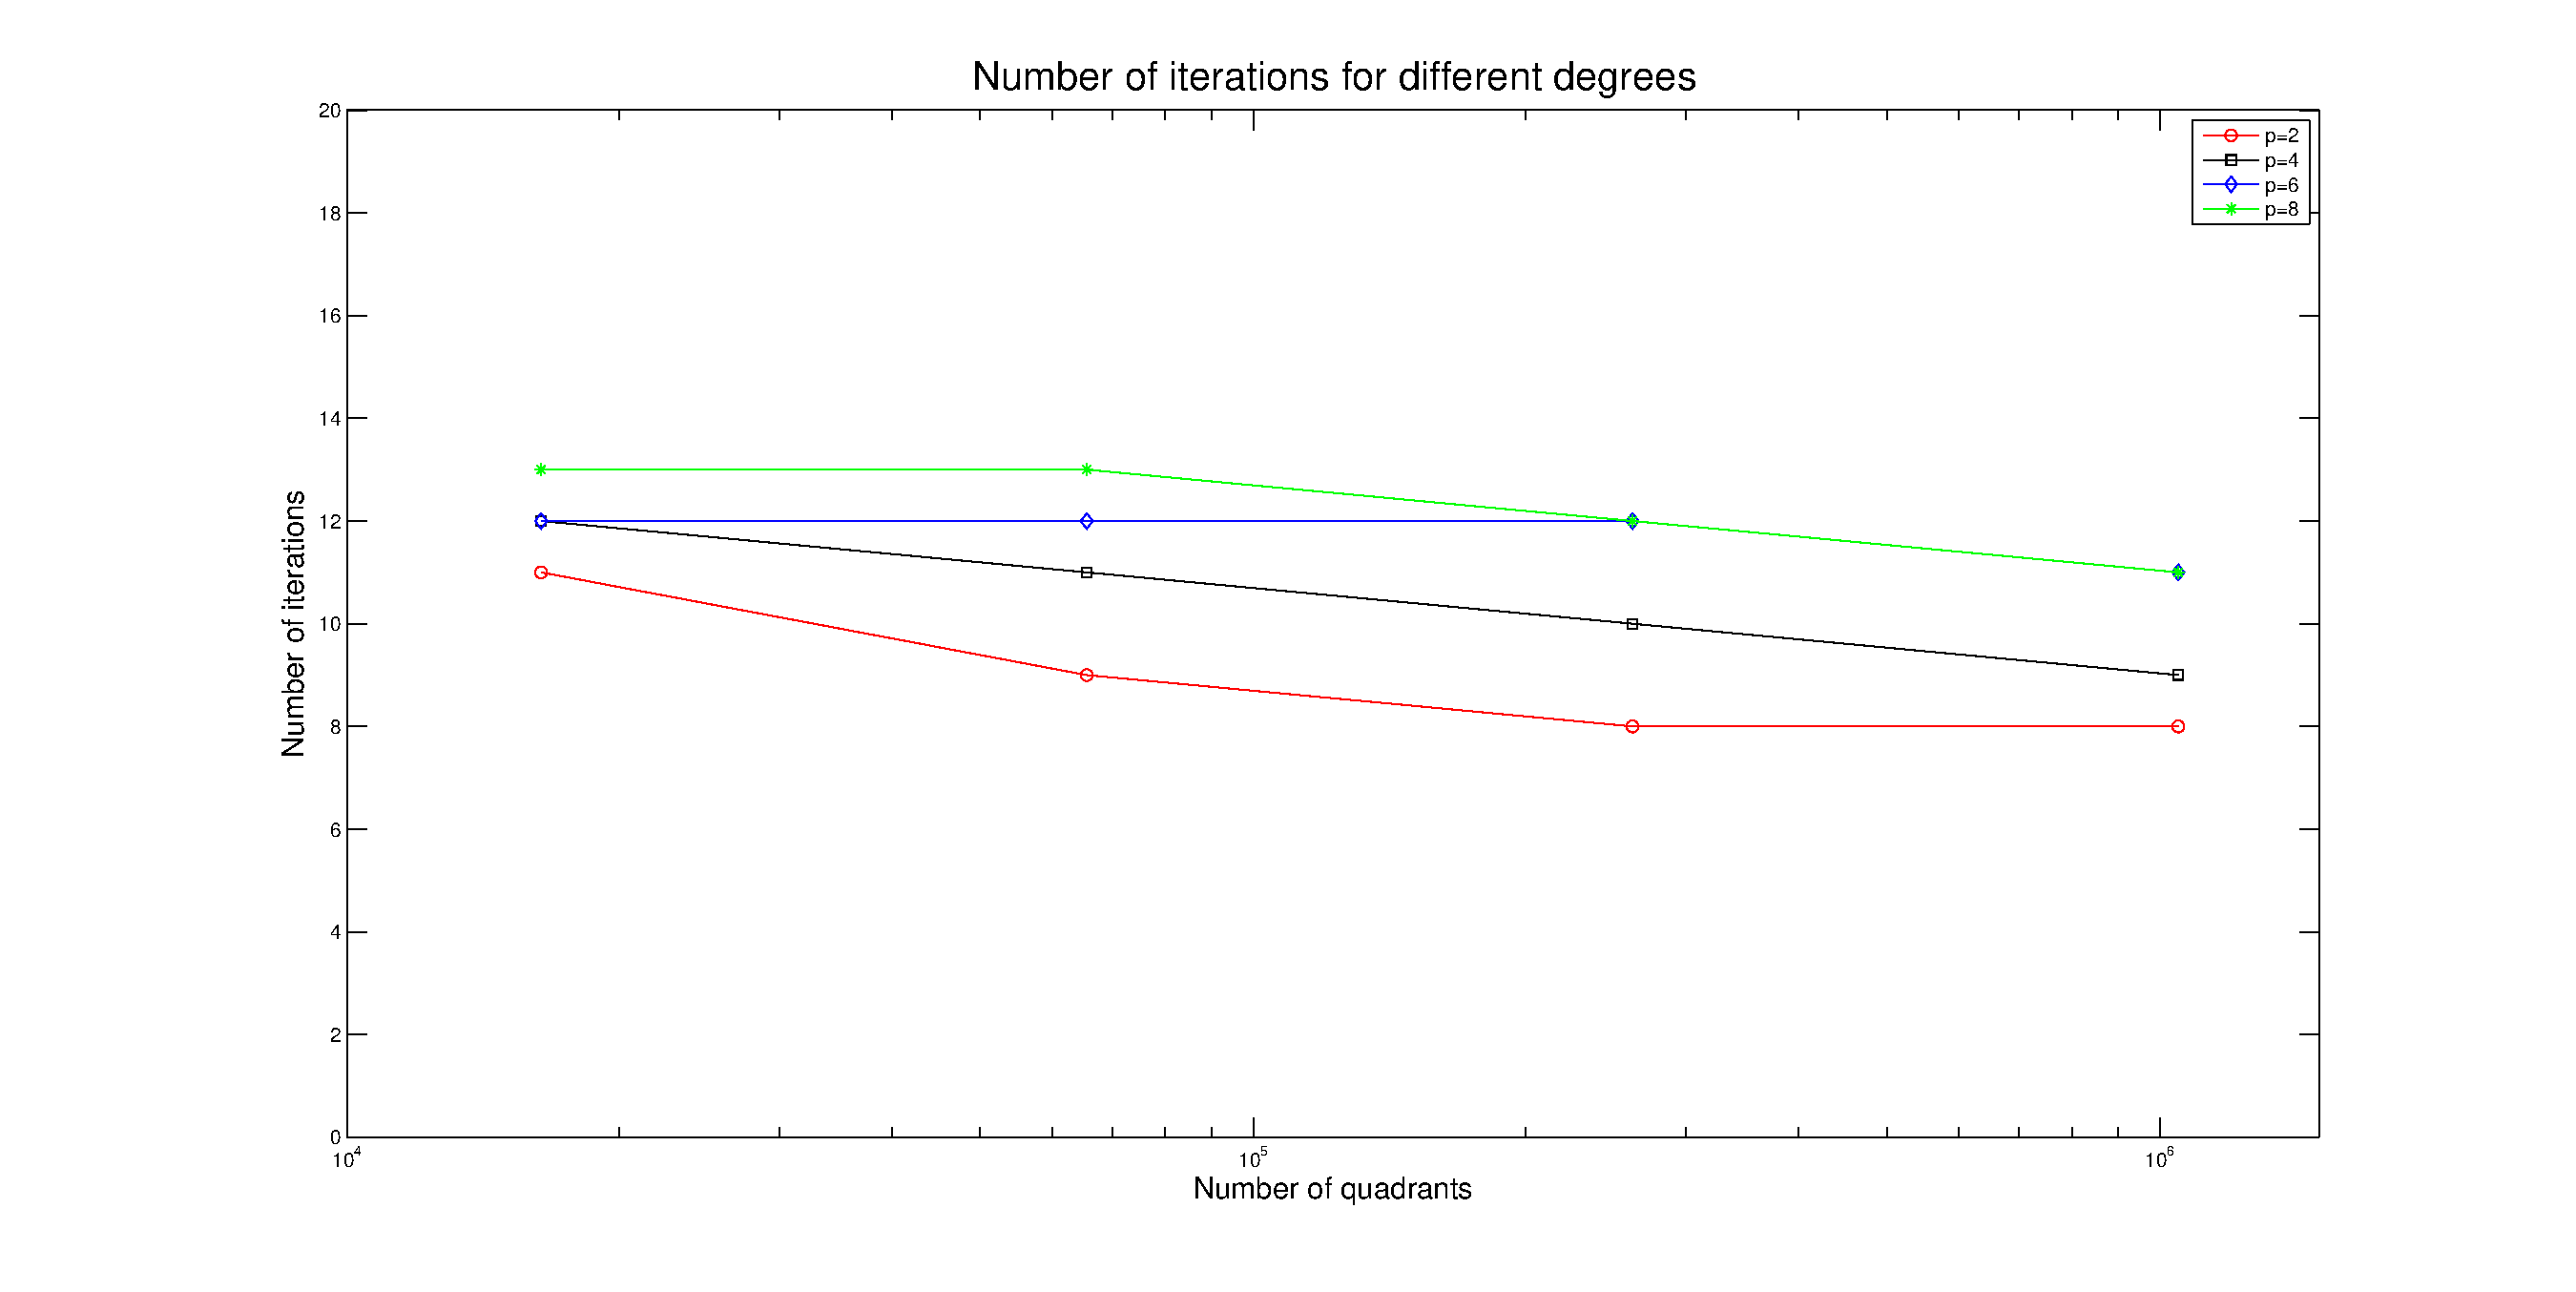
\includegraphics[scale=0.35]{Results/two_reg_iter.eps}
\caption{Number of iterations of PCG with the two scale preconditioner for degree $p$ of interpolation needed to reach the given tolerance of the norm of the residual as a function of the number of quadrants in a regular mesh.}
\label{two_reg_iter}
\end{figure}

For the following tests, we also have tighten the tolerance on the norm of the residual. We now require that : 

$$\frac{||r_k||_2}{||r_0||_2} < 10^{-5}$$

Figure \ref{two_reg_iter} shows the number of iterations needed to reach that tolerance of the norm of the residual when we use our two scale preconditioner for different degrees of interpolation. The first remark we can make is that the number of iterations does not increase with the number of quandrants (as it was the case when we only had the fine preconditioner). So we can conclude that the coarse preconditioner does the job it was designed to do. We can even note that the number of iterations slightly decreases. For example, for $p=6$, we need 12 iterations for $128^2$ quadrants but we only do 11 iterations for $1024^2$. An explanation for this phenomenon might be that when we increase the number of quadrants, we actually better separate the actions of the fine and coarse preconditioners and therefore the sum of the two is a better approximation of $A^{-1}$. We can mention that for $p=8$, we only need 11 iterations to solve a system that has more than 67 millions unknowns. 

A second remark we can make, as already observed when we only had the fine preconditioner, is that the number of iterations grows with the degree of the interpolation. For example, with $1024^2$ quadrants, we need 8 iterations when $p=2$ but we need to do 11 iterations when $p=8$. As before, this can be explained by the fact that as the degree of the interpolation increases, the size of the overlap decreases. A fixed sized overlap would fix this issue. 

\subsubsection{Meshes with distorted elements}

We will now look at what happens when the mesh is not regular but we have quadrants that are more and more distorted. We will use the same meshes already used in the previous section and obtained with the progression tool of GMSH (see figure \ref{fine_mesh_deform} for example of such meshes).

\begin{figure}
\centering
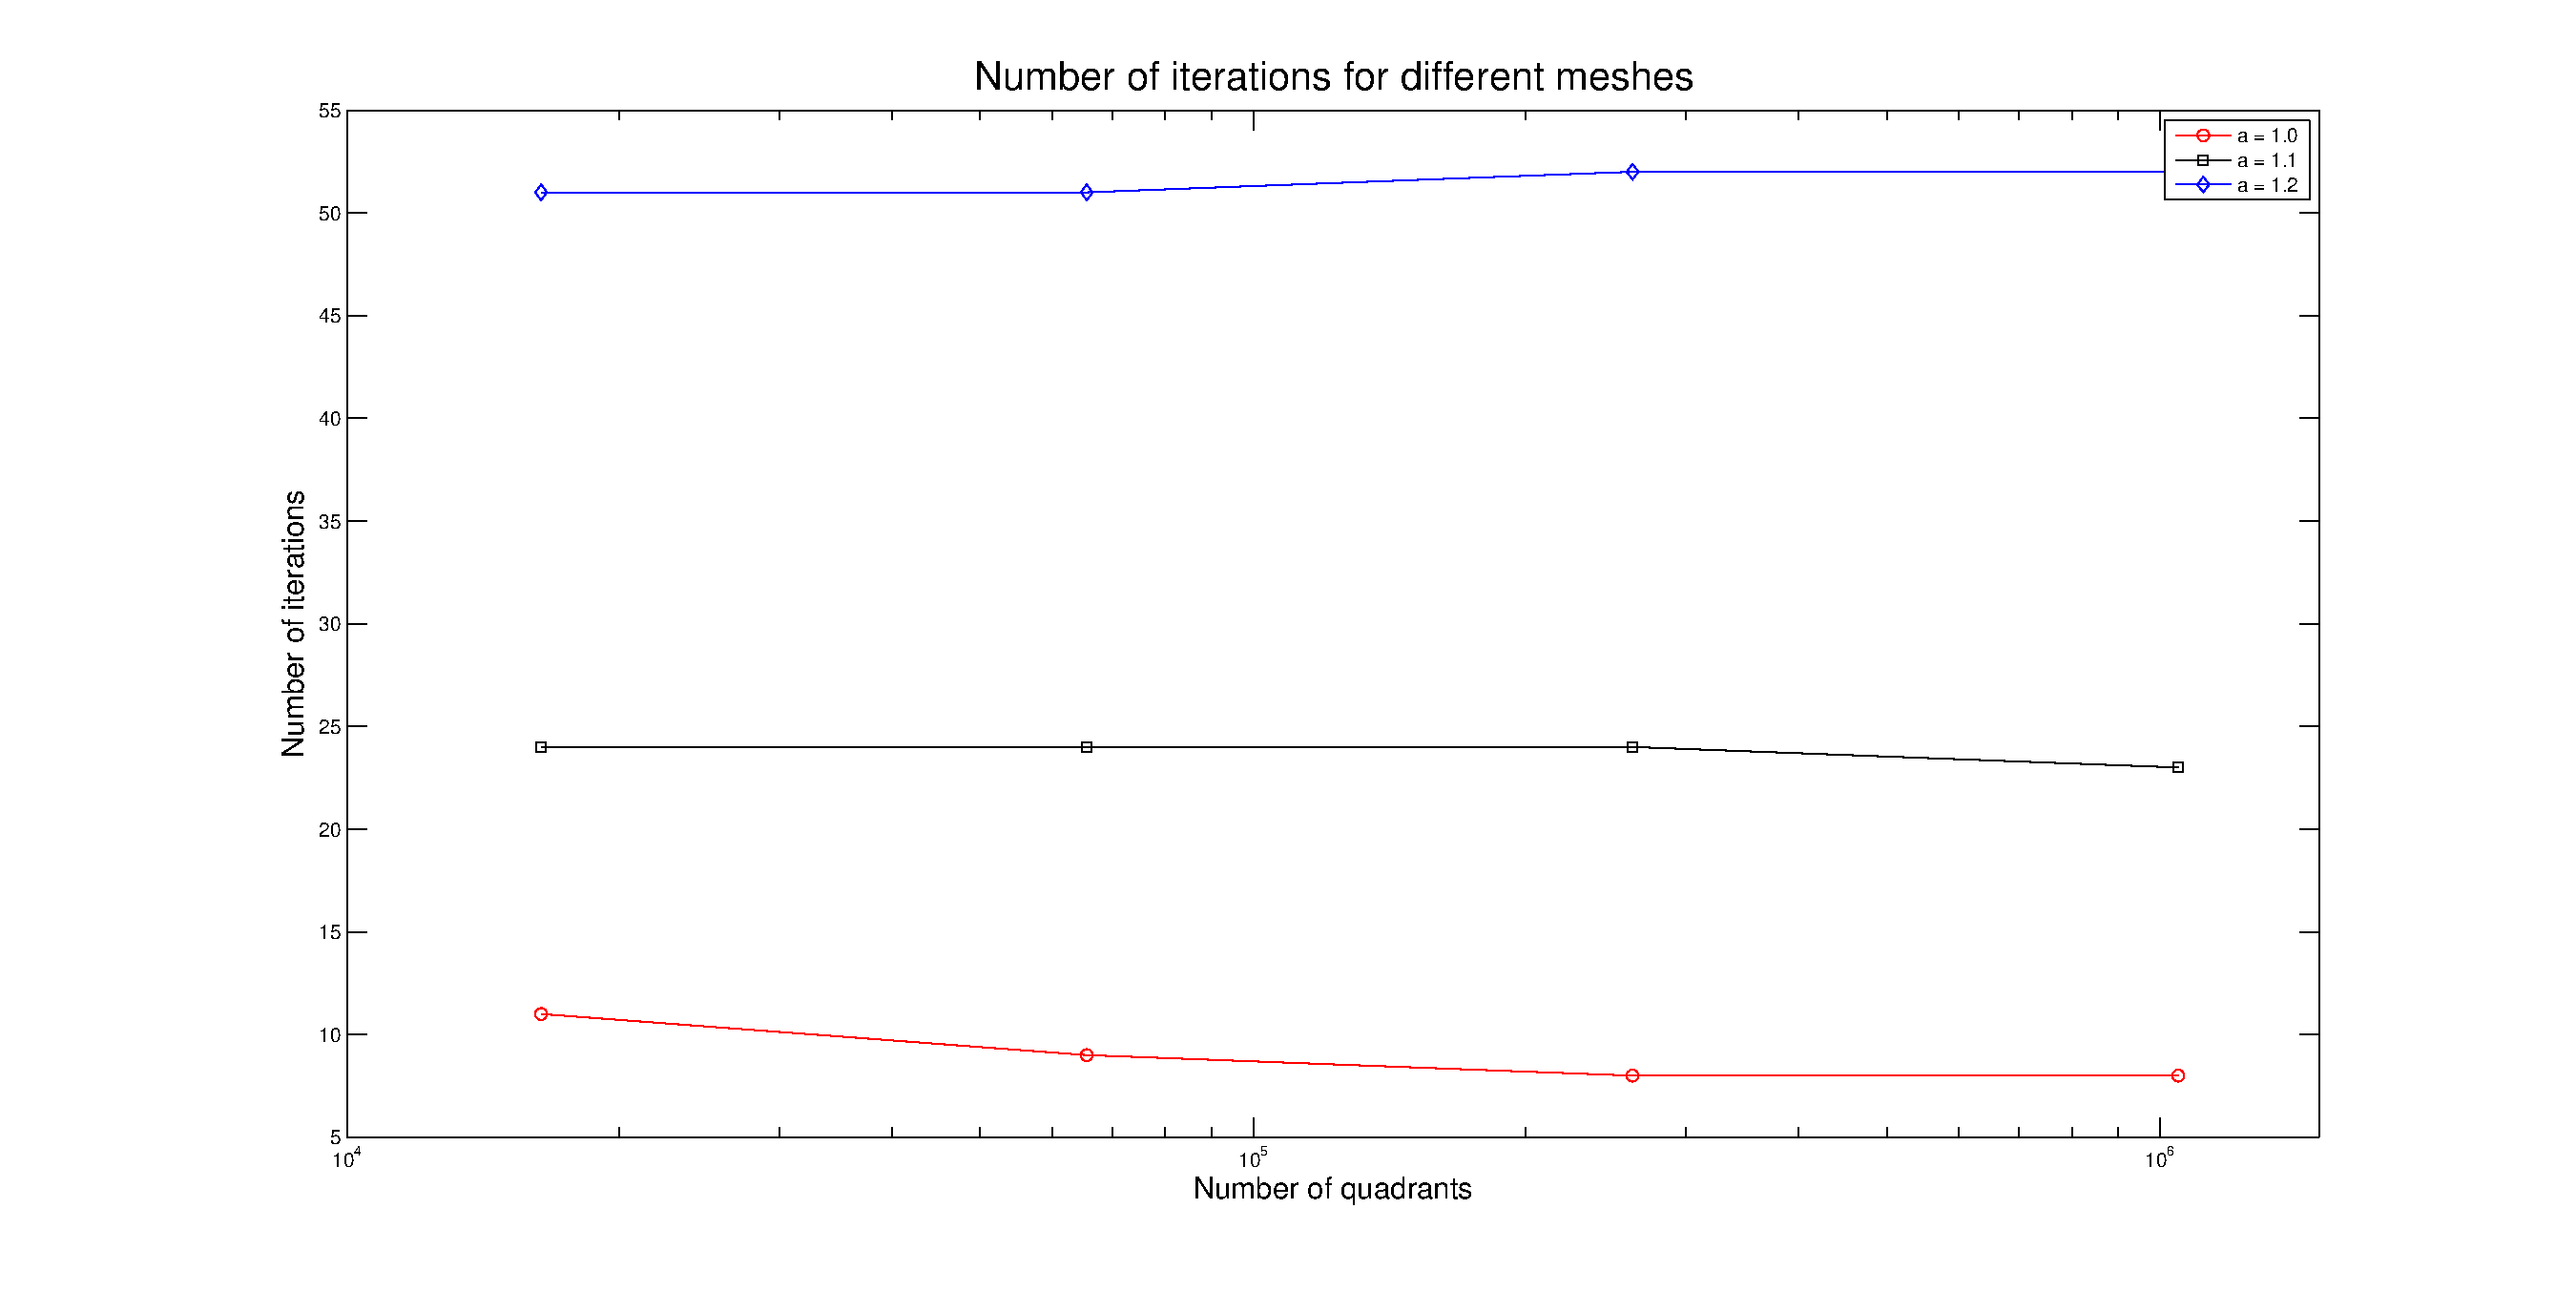
\includegraphics[scale=0.35]{Results/two_irreg_iter.eps}
\caption{Number of iterations of PCG with the two scale preconditioner for an interpolation degree $p=2$ needed to reach the given tolerance on the norm of the residual as a function of the number of quadrants for meshes with quadrants more and more distorted.}
\label{two_irreg_iter}
\end{figure}

For an interpolation of degree $p=2$, we looked at the number of iterations needed to reach the given tolerance as we increase the number of quadrants and for elements more and more distorted. Figure \ref{two_irreg_iter} shows the results. We can see that the number of iterations stays roughly the same when we increase the number of quadrants so once again the coarse part of the preconditioner does the job it is designed to do. 

We can also node that when the more we distort the quadrants the more iterations we need to reach the given tolerance. This is to be expected since we developed the fine preconditioner to work optimally on quadrants aligned with the axis. This means that the more a quadrant is distorted the less accurate is the fine preconditioner part and therefore the more iterations we need. However, even with the most distorted mesh, the number of iterations stays acceptable and as explained in the previous section, the gain of not having to solve exactly on every quadrant is huge. We also have to say that the meshes presented here have an intrinsic structure since they are generated using the progression tool in GMSH. Therefore, the errors we make with our approximation are always in the same direction and the number of iterations needed increases. We might not have such an increase with a random mesh containing quadrants with the same quality measure. 

\textcolor{red}{Ajouter ici un mesh random si espace dispo}

\subsection{Influence of hanging nodes}

Let us now move on to the cases when we have hanging nodes. As in the part with only the fine preconditioner, we will look at a problem where the solution has a jump so that we create hanging nodes when we use a recursive refine function in p4est. In addition to the hyperbolic tangent already presented in the previous subsection, we will include a high frequency sine wave to see how the grid adapts to capture it and how the two scale preconditioner performs in its presence. 

The problem we will solve is : 

\begin{align}
\nabla^2 u =& -2\tanh(12x)\tanh(12y)\left[ 12^2(1-\tanh(12x)^2) + 12^2(1-\tanh(12y)^2)\right] \nonumber \\
 &-  10\pi^2\sin(10\pi x)\sin(10\pi y) &\text{on $\Omega$} \label{eq:two_hang}\\
u =&   \tanh(12x)\tanh(12y) + \frac{1}{20}\sin(10\pi x)\sin(10\pi y)&\text{on $\Gamma$}
\end{align}

Where $\Omega = [-1;1]^2$ and $\Gamma$ is the boundary. This problem has an analytic solution that is given by : 

$$u(x,y) = \tanh(12x)\tanh(12y) + \frac{1}{20}\sin(10\pi x)\sin(10\pi y)$$

\begin{figure}
\centering
\includegraphics[scale=0.35]{Results/two_hang_plot.eps}
\caption{Numerical solution to problem \ref{eq:two_hang} using an interpolation of order $p=2$ on a non conforming mesh and obtained with PCG with the two scale preconditioner.}
\label{two_hang_plot}
\end{figure}

Figure \ref{two_hang_plot} shows an example of the numerical solution computed on a non conforming mesh with PCG and the two scale preconditioner. We can see on the plot both the steep jump due to the hyperbolic tangent and the small oscillations due to the sine wave.

\subsubsection{Increasing the relative number of hanging nodes}

